\documentclass[11pt]{article}
\usepackage[a4paper,margin=1in]{geometry}
\usepackage{amsmath,amssymb,amsthm,mathtools}
\usepackage{graphicx}
\usepackage{xcolor}
\usepackage{microtype}
\usepackage{enumitem}
\usepackage[colorlinks=true,linkcolor=blue!55!black,citecolor=blue!55!black,urlcolor=blue!55!black]{hyperref}
\setlength{\emergencystretch}{1em}

\newtheorem{theorem}{Theorem}
\newtheorem{proposition}[theorem]{Proposition}
\newtheorem{lemma}[theorem]{Lemma}
\theoremstyle{definition}
\newtheorem{definition}[theorem]{Definition}
\newtheorem{remark}[theorem]{Remark}

\newcommand{\C}{\mathbb C}
\newcommand{\N}{\mathbb N}
\newcommand{\Q}{\mathbb Q}
\newcommand{\T}{\mathbb T}
\newcommand{\Orb}{\operatorname{Orb}}
\newcommand{\dist}{\operatorname{dist}}
\newcommand{\Gamstar}{\Gamma_{\!*}}

\title{One Countable Non-Dense Scalar Set for Every\\
Nonexceptional Supercyclic Spectral Class}
\author{Candidate sharp spectral theorem for arXiv:1509.04912}
\date{9 August 2026}

\begin{document}
\maketitle

\begin{center}
\fcolorbox{blue!55!black}{blue!4}{\parbox{0.91\linewidth}{
\textbf{Status.} Candidate full theorem, likely valid; human review
recommended. It gives a sharp maximal spectral partial answer to Question~3:
one explicit countable non-dense scalar set works in every supercyclic
adjoint-spectral class except $\{1\}$, and no non-dense set can cover that
last class uniformly. It does not characterize every admissible scalar set.}}
\end{center}

\section{Source problem}

The source is S.~Charpentier, R.~Ernst, and Q.~Menet,
\emph{$\Gamma$-supercyclicity}, arXiv:1509.04912 \cite{CEM}. For
$T\in\mathcal L(X)$, a vector $x$ is $\Gamma$-supercyclic when
\[
  \Orb(\Gamma x,T)=\{\gamma T^n x:\gamma\in\Gamma,\ n\geq0\}
\]
is dense in $X$. Question~3 asks which $\Gamma\subset\C$ make
supercyclicity equivalent to $\Gamma$-supercyclicity.

\begin{figure}[ht]
  \centering
  
\includegraphics[width=\linewidth]{figures/open_problem_crop.png}
  \caption{Question~3 on page 3 of the source paper.}
\end{figure}

The source exactly treats each unimodular adjoint eigenvalue in Theorem~C,
but explicitly leaves the nonunit and empty-adjoint-point-spectrum regimes
unclear.  The theorem below fills all of those regimes at once with the same
small scalar set and simultaneously handles every unimodular eigenvalue
except the uniquely unavoidable value $1$.

\begin{figure}[ht]
  \centering
  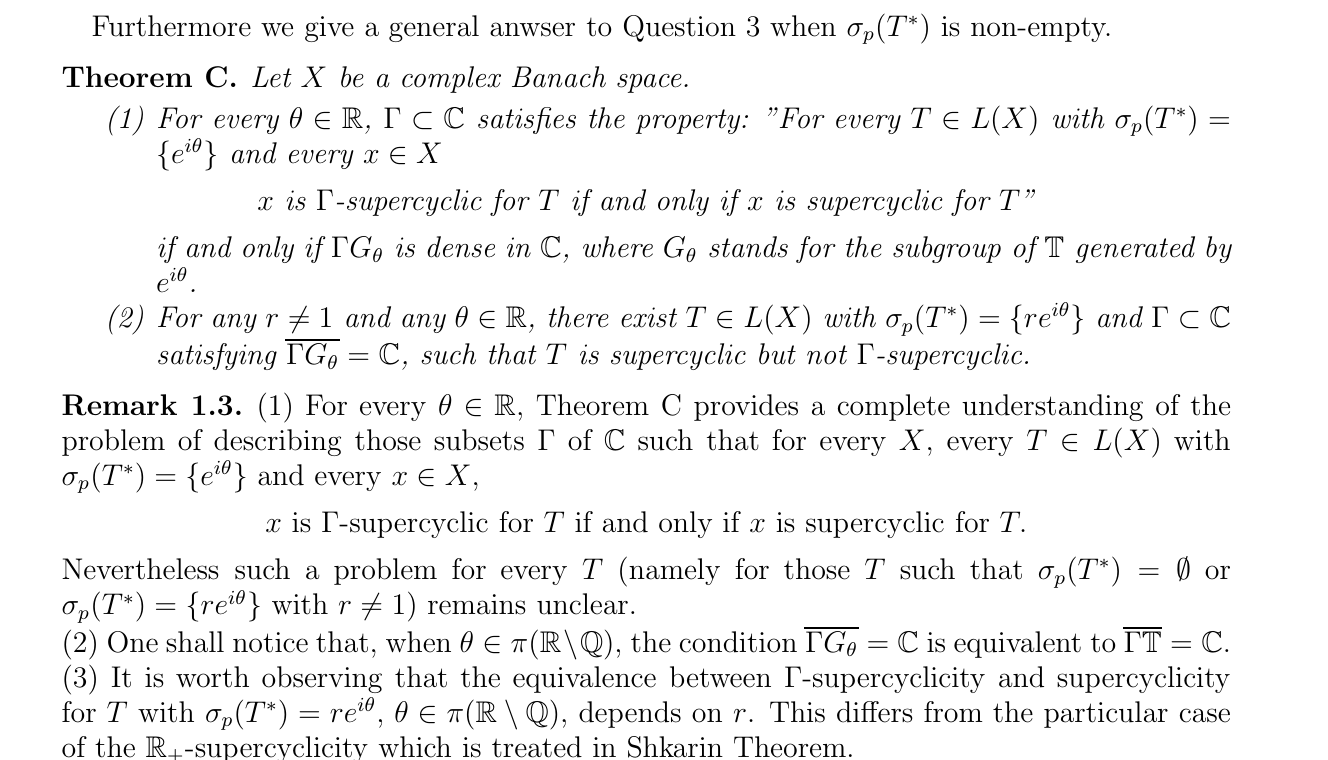
\includegraphics[width=\linewidth]{figures/residual_case_crop.png}
  \caption{Theorem~C and the unresolved regimes on page 4 of the source.}
\end{figure}

\clearpage
\section{Statement and proof intuition}

Write $\Q(i)=\Q+i\Q$, and set
\begin{equation}\label{eq:gamma-star}
 \Gamstar=\Q(i)\cap\bigl(
 \{z:|z|<1\}\cup\{z:|z|>2\}\cup\{z:\Re z>0\}\bigr).
\end{equation}

\subsection*{Proof intuition}

The three pieces of \eqref{eq:gamma-star} match the three possible
adjoint-spectral regimes of a supercyclic operator.  When the point spectrum
is empty, positive and ordinary supercyclic vectors coincide; positive
rationals already suffice and lie in $\Gamstar$.  When the eigenvalue is
nonunit, the backward-scaled target $\mu^{-n}c$ eventually lies in the inner
disk or the exterior region, where Gaussian rationals approximate it with
arbitrarily fine relative accuracy.  When the eigenvalue is unimodular and
not $1$, the cyclic rotations of a half-plane cover the whole plane, exactly
matching the source's phase-group criterion.

The omitted value $1$ is not a weakness of the construction.  Theorem~C of
the source says that a scalar set working uniformly in that class must itself
be dense.  Hence $\{1\}$ is the unique spectral class that every non-dense
uniform construction must exclude.

\begin{theorem}[Maximal non-dense spectral coverage]\label{thm:main}
Let $X$ be an infinite-dimensional complex Banach space.  For every
$T\in\mathcal L(X)$ satisfying $\sigma_p(T^*)\ne\{1\}$ and every $x\in X$,
\[
 x\text{ is supercyclic for }T
 \quad\Longleftrightarrow\quad
 x\text{ is $\Gamstar$-supercyclic for }T.
\]
The set $\Gamstar$ is countable and non-dense in $\C$.

Moreover, the exclusion is sharp: if $\Lambda\subset\C$ has the displayed
equivalence uniformly for all operators in the class
$\sigma_p(T^*)=\{1\}$, then $\Lambda$ is dense in $\C$.
\end{theorem}

The adjoint convention in \cite{CEM} conjugates eigenfunctional multipliers.
This causes no ambiguity here: modulus is preserved, $1$ is fixed, and a
unimodular scalar and its conjugate generate the same cyclic subgroup.

\section{A common tail-universal set for every nonunit multiplier}

\begin{definition}
For $\mu\in\C\setminus\{0\}$, a set $\Gamma\subset\C$ is
\emph{tail-universal for $\mu$} if
\begin{equation}\label{eq:tail}
 \forall c\in\C,\qquad \dist(c,\mu^n\Gamma)\longrightarrow0.
\end{equation}
\end{definition}

\begin{lemma}[Universal annular-gap set]\label{lem:common-tail}
The set $\Gamstar$ is tail-universal for every $\mu\ne0$ with
$|\mu|\ne1$.
\end{lemma}

\begin{proof}
Fix $c\in\C$.  If $c=0$, use $0\in\Gamstar$.  Suppose $c\ne0$ and put
$z_n=\mu^{-n}c$.  If $|\mu|>1$, then $z_n$ eventually belongs to the open
unit disk.  By density of $\Q(i)$, choose $\gamma_n\in\Q(i)$ in that disk
with
\[
 |\gamma_n-z_n|<\frac{|\mu|^{-n}}{n}.
\]
Then $\gamma_n\in\Gamstar$ and
$|\mu^n\gamma_n-c|<1/n$.  If $|\mu|<1$, then $|z_n|>2$ eventually; choose
the same approximation inside the open region $\{|z|>2\}$.  The identical
estimate proves \eqref{eq:tail}.
\end{proof}

\begin{lemma}[Projective tails]\label{lem:tails}
If $x$ is supercyclic for $T$, then
$\bigcup_{n\geq N}\C T^n x$ is dense in $X$ for every $N\geq0$.
\end{lemma}

\begin{proof}
Otherwise some nonempty open set would miss one tail.  Density of the full
projective orbit would then force a finite union of one-dimensional closed
subspaces to be dense in that open set.  Being closed, that finite union
would contain the open set, contradicting that a finite union of proper
linear subspaces has empty interior.
\end{proof}

\begin{proposition}[Tail transfer]\label{prop:transfer}
Suppose $f\circ T=\mu f$ for some $f\in X^*\setminus\{0\}$ and $\mu\ne0$.
If $\Gamma$ is tail-universal for $\mu$, then every supercyclic vector for
$T$ is $\Gamma$-supercyclic.
\end{proposition}

\begin{proof}
Let $x$ be supercyclic.  Necessarily $f(x)\ne0$.  Fix $y$ with $f(y)\ne0$.
Lemma~\ref{lem:tails} gives $n_k\geq k$ and $\alpha_k\in\C$ such that
$\alpha_kT^{n_k}x\to y$.  Applying $f$ yields
\[
 \alpha_k\mu^{n_k}\longrightarrow c:=\frac{f(y)}{f(x)}\ne0.
\]
Tail universality supplies $\gamma_k\in\Gamma$ with
$\gamma_k\mu^{n_k}\to c$.  Hence
\[
 \frac{\gamma_k}{\alpha_k}
 =\frac{\gamma_k\mu^{n_k}}{\alpha_k\mu^{n_k}}\longrightarrow1,
\]
so $\gamma_kT^{n_k}x\to y$.  Thus the closure of the $\Gamma$-orbit
contains $X\setminus\ker f$, a dense set.
\end{proof}

\section{Unimodular and empty-spectrum regimes}

\begin{lemma}[Rotated half-planes]\label{lem:halfplanes}
If $\lambda\in\T\setminus\{1\}$ and $G_\lambda$ is the cyclic subgroup
generated by $\lambda$, then $\overline{\Gamstar G_\lambda}=\C$.
\end{lemma}

\begin{proof}
The set $\Gamstar$ is dense in the open right half-plane, so its closure
contains the closed right half-plane $H=\{z:\Re z\geq0\}$.  If $\lambda$
has finite order $q\geq2$, the $q$ directions in $G_\lambda$ have angular
gaps $2\pi/q$; every direction is within $\pi/q\leq\pi/2$ of one of them.
Thus $\bigcup_{g\in G_\lambda}gH=\C$.  If $\lambda$ has infinite order,
$G_\lambda$ is dense in $\T$ and the same conclusion is immediate.
Therefore the closure of $\Gamstar G_\lambda$ is all of $\C$.
\end{proof}

\begin{lemma}[Positive rational reduction]\label{lem:rational}
If $x$ is $\mathbb R_+$-supercyclic for $T$, then $x$ is
$\Q_+$-supercyclic, and hence $\Gamstar$-supercyclic.
\end{lemma}

\begin{proof}
The positive projective orbit is dense.  Whenever $tT^nx$ lies in a chosen
open set, continuity of $s\mapsto sT^nx$ and density of $\Q_+$ in
$\mathbb R_+$ allow $t$ to be replaced by a positive rational.  Finally
$\Q_+\subset\Gamstar$.
\end{proof}

\section{Proof of the main theorem}

\begin{proof}[Proof of Theorem~\ref{thm:main}]
Countability of $\Gamstar$ is immediate.  Moreover
\[
 \overline{\Gamstar}\subset
 \{|z|\leq1\}\cup\{|z|\geq2\}\cup\{\Re z\geq0\},
\]
so it misses the nonempty open half-annulus
$\{1<|z|<2,\ \Re z<0\}$ and is not dense.

Since $\Gamstar\subset\C$, every $\Gamstar$-supercyclic vector is
supercyclic.  Conversely, let $x$ be supercyclic for $T$.  The classical
adjoint-spectrum dichotomy says that $\sigma_p(T^*)$ is empty or is a
singleton $\{\eta\}$ with $\eta\ne0$ \cite{Shkarin}.

If it is empty, Proposition LM of \cite{Shkarin} (the
Le\'on-Saavedra--M\"uller theorem) says that the supercyclic and
$\mathbb R_+$-supercyclic vectors coincide.  Lemma~\ref{lem:rational}
applies.

Suppose $\sigma_p(T^*)=\{\eta\}$.  If $|\eta|\ne1$, the corresponding
eigenfunctional multiplier has nonunit modulus, so
Lemma~\ref{lem:common-tail} and Proposition~\ref{prop:transfer} apply.  If
$|\eta|=1$, the hypothesis gives $\eta\ne1$; Lemma~\ref{lem:halfplanes}
and the exact unimodular characterization in Theorem~C(1) of \cite{CEM}
give that $x$ is $\Gamstar$-supercyclic.

For sharpness, apply the necessity direction of Theorem~C(1) in \cite{CEM}
at $\eta=1$.  The generated phase group is $\{1\}$, so uniform equivalence
in this spectral class holds only if $\overline\Lambda=\C$.
\end{proof}

\section{Verification, novelty, and scope}

The proof is analytic.  The accompanying script checks representative
nonunit rescalings and finite cyclic half-plane covers; it is not used as
proof.

A bounded search on 9 August 2026 covered:
\begin{itemize}[nosep,leftmargin=1.4em]
\item the run indexes and arXiv:1509.04912, 1209.1222, 1711.10932, and
  2411.03179;
\item arXiv queries combining \emph{$\Gamma$-supercyclicity},
  \emph{countable non-dense scalar set}, \emph{point spectrum},
  \emph{annulus}, and \emph{half-plane}.
\end{itemize}
No statement using one countable non-dense set for every spectral class
except the sharp eigenvalue-one obstruction was found.  Novelty confidence
is moderate.

This is a complete and sharp maximal spectral-coverage theorem.  It remains
a partial answer to Question~3 because it does not characterize all scalar
sets for each nonunit eigenvalue or in the empty-spectrum regime.  Human
review should focus on the three cited spectral inputs, the common
tail-universality argument, and the novelty assessment.

\begin{thebibliography}{9}
\bibitem{CEM}
S.~Charpentier, R.~Ernst, and Q.~Menet,
\emph{$\Gamma$-supercyclicity}, arXiv:1509.04912 (2015).

\bibitem{Shkarin}
S.~Shkarin,
\emph{Universal elements for non-linear operators and their applications},
J. Math. Anal. Appl. 348 (2008), 193--210; arXiv:1209.1222.
\end{thebibliography}

\end{document}
